
\begin{figure}
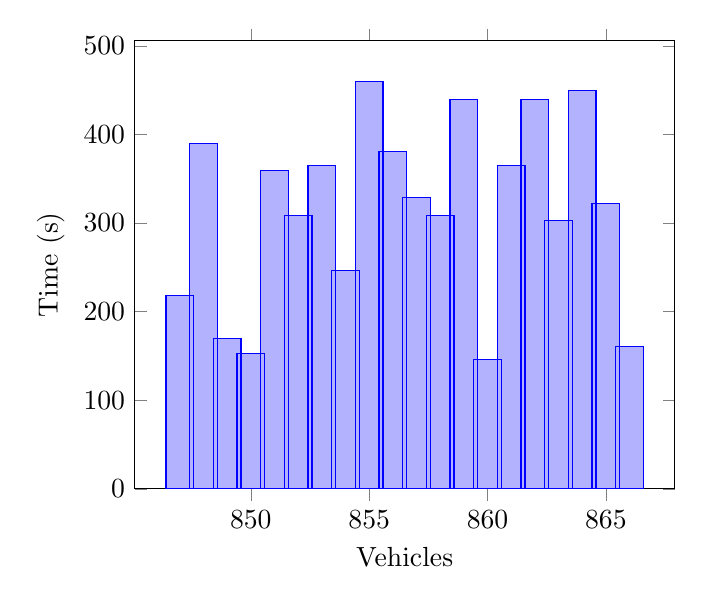
\begin{tikzpicture}
\begin{axis}[
legend style={anchor=west},
xlabel=Vehicles,
ylabel=Time (s),
ymin=0,
ybar,
]
\addplot coordinates {
(852, 308)
(858, 308)
(849, 170)
(859, 439)
(850, 153)
(847, 218)
(851, 359)
(866, 161)
(864, 450)
(854, 246)
(853, 365)
(865, 322)
(855, 460)
(856, 381)
(857, 329)
(862, 439)
(860, 146)
(861, 365)
(848, 390)
(863, 303)
};

\end{axis}
\end{tikzpicture}
\label{tik:time:100:25}
\caption{100 percent diving with GSC on route $25$}
\end{figure}
